\documentclass{beamer}
\usepackage{beamerthemeshadow}
\usepackage{beamercolorthemeucf}
\usepackage[ruled]{algorithm}
\usepackage{listings}
%\usepackage[font=scriptsize]{subcaption}
\usepackage[font=scriptsize]{caption}
\usepackage[noend]{algpseudocode}
\usepackage[hyperref=true,style=numeric,defernumbers,backend=bibtex,sorting=ydnt,maxnames=6,sortcites=true]{biblatex}
\usepackage{slashbox}
\usepackage{tabularx}
\usepackage{booktabs}

\addbibresource{citation.bib}
\DeclareBibliographyCategory{Journal}
\DeclareBibliographyCategory{Conference}
\DeclareBibliographyCategory{Workshop}
\addtocategory{Journal}{sottile2014static,zhang2015validating,zhang2015lockfree,zhang2014queue}
\addtocategory{Conference}{zhang2014tools,zhang2013fast,zhang2016lockfree,zhang2016efficient,zhang2016highperformance}
\addtocategory{Workshop}{feldman2015extending,peterson2014resourse}

\mode<presentation>

\useinnertheme[shadow=true]{rounded}
\useoutertheme{infolines}
\usecolortheme{ucf}

\setbeamertemplate{sections/subsections in toc}[square]
\setbeamertemplate{items}[square]

\setbeamertemplate{footline}
{
  \leavevmode%
  \hbox{%
  \begin{beamercolorbox}[wd=.3\paperwidth,ht=2.25ex,dp=1ex,center]{author in head/foot}%
      \usebeamerfont{author in head/foot}\insertshortauthor{}
  \end{beamercolorbox}%
  \begin{beamercolorbox}[wd=.4\paperwidth,ht=2.25ex,dp=1ex,center]{title in head/foot}%
    \usebeamerfont{title in head/foot}\insertshorttitle
  \end{beamercolorbox}%
  \begin{beamercolorbox}[wd=.3\paperwidth,ht=2.25ex,dp=1ex,right]{date in head/foot}%
    \usebeamerfont{date in head/foot}\insertshortdate{}\hspace*{2em}
    \insertframenumber{} / \inserttotalframenumber\hspace*{2ex} 
  \end{beamercolorbox}}%
  \vskip0pt%
}
\settowidth{\leftmargini}{\usebeamertemplate{itemize item}}
\addtolength{\leftmargini}{\labelsep}

\renewcommand{\thefootnote}{\fnsymbol{footnote}}
\setbeamerfont{footnote}{size=\tiny}
\captionsetup[figure]{labelformat=empty}
\graphicspath{ {./figure/} }

\lstset{
    language=C++, 
    numbers=none, 
    numbersep=10pt,
    numberstyle=\small, 
    xleftmargin=0pt, 
    basicstyle=\scriptsize\ttfamily,
    commentstyle=\scriptsize\itshape\sffamily,
    showstringspaces=false, 
    tabsize=2, 
    breaklines=true, 
    morecomment=[l]{//}
}

\begin{document}
\title[Lock-free Transactional Transformation]{Lock-free Transactions without Rollbacks for Linked Data Structures}
\author[D. Zhang and D. Dechev]{\underline{Deli Zhang} and Damian Dechev}
\institute{Department of Computer Science\\ 
University of Central Florida}

\date[SPAA 2016]{28th ACM Symposium on Parallelism in Algorithms and Architectures}

\begin{frame}
    \titlepage
\end{frame}

%\begin{frame}
    %\frametitle{Table of Contents}
    %\tableofcontents
%\end{frame}

\section{Introduction}
\subsection{Motivation}
%\begin{frame} \frametitle{Many-core Processors Are Here}
    %\begin{columns}
        %\begin{column}{5cm}
            %\begin{itemize}
                %\item Intel Xeon Phi 7290 
                %\item 72 x86 cores
                %\item<2> Sunway SW26010
                %\item<2> 260 RISC cores
            %\end{itemize}
        %\end{column}
        %\begin{column}{7cm}
            %\begin{figure}[H]
                %\centering
                %\includegraphics<1->[width=1\textwidth]{xeon7290}
            %\end{figure}
        %\end{column}
    %\end{columns}
%\end{frame}

%\begin{frame} \frametitle{Non-blocking Data Structures}
    %\begin{columns}
        %\begin{column}{5cm}
            %\begin{itemize}
                %\item<1-> Progress Guarantees
                    %\begin{itemize}
                        %\item Wait-freedom
                        %\item Lock-freedom
                        %\item Obstruction-freedom
                    %\end{itemize}
            %\end{itemize}
        %\end{column}
        %\begin{column}{5cm}
            %\begin{itemize}
                %\item<1-> Linearizability
                    %\begin{itemize}
                        %\item Compositional
                        %\item Container libraries
                        %\item LibCDS, Tervel, TBB
                    %\end{itemize}
            %\end{itemize}
        %\end{column}
    %\end{columns}
    %\begin{example}<2>
        %\lstinputlisting[basicstyle=\footnotesize,language=JAVA]{./code/move.java}
    %\end{example}
%\end{frame}

\begin{frame} \frametitle{Composite Operations}
\begin{example}<1->
        \lstinputlisting[basicstyle=\footnotesize,language=JAVA]{./code/move.java}
\end{example}
\begin{example}<2->
        \lstinputlisting[basicstyle=\small,language=JAVA]{./code/insertifcontain.java}
\end{example}
\begin{itemize}
    \item<3> Composing linearizable operations is error-prone \textcolor{gray}{[Shacham et al., 2011]}
        %\begin{itemize}
                %\item Expose internal locks --- break encapsulation
                %\item Manual composition --- state explosion
        %\end{itemize}
    \end{itemize}
\end{frame}

\begin{frame} \frametitle{Transactional Data Structures}
            \begin{block}{Atomicity}
                If one operation fails, the entire transaction should abort.
            \end{block}
            \begin{block}{Isolation} 
                Concurrent execution of transactions appears to take effect in some sequential orders that respect real-time ordering.
            \end{block}
        %\item Strict serializability
            %\begin{itemize}
                %\item Analogue of linearizability for transactions
            %\end{itemize}
\end{frame}

\subsection{Related Work}
\begin{frame} \frametitle{Software Transactional Memory (STM)}
    \begin{block}{}
        \small
        An STM instruments threads' memory accesses, which records the locations a thread read in a \emph{read set}, and the locations it writes in a \emph{write set}. Conflicts are detected among the \emph{read/write sets} of different threads. In the presence of conflicts, only one transaction is allowed to commit while the others are aborted and restarted.
    \end{block}
    \begin{itemize}
        \item<1-> Memory instrumentation exhibits large overhead
        \item<2> Low-level memory conflicts do not translate to high-level semantic conflicts, which cause excessive aborts
    \end{itemize}
\begin{overlayarea}{\textwidth}{.40\textheight}
        \centering
        \visible<2>{
    \begin{figure}[h]
        \centering
        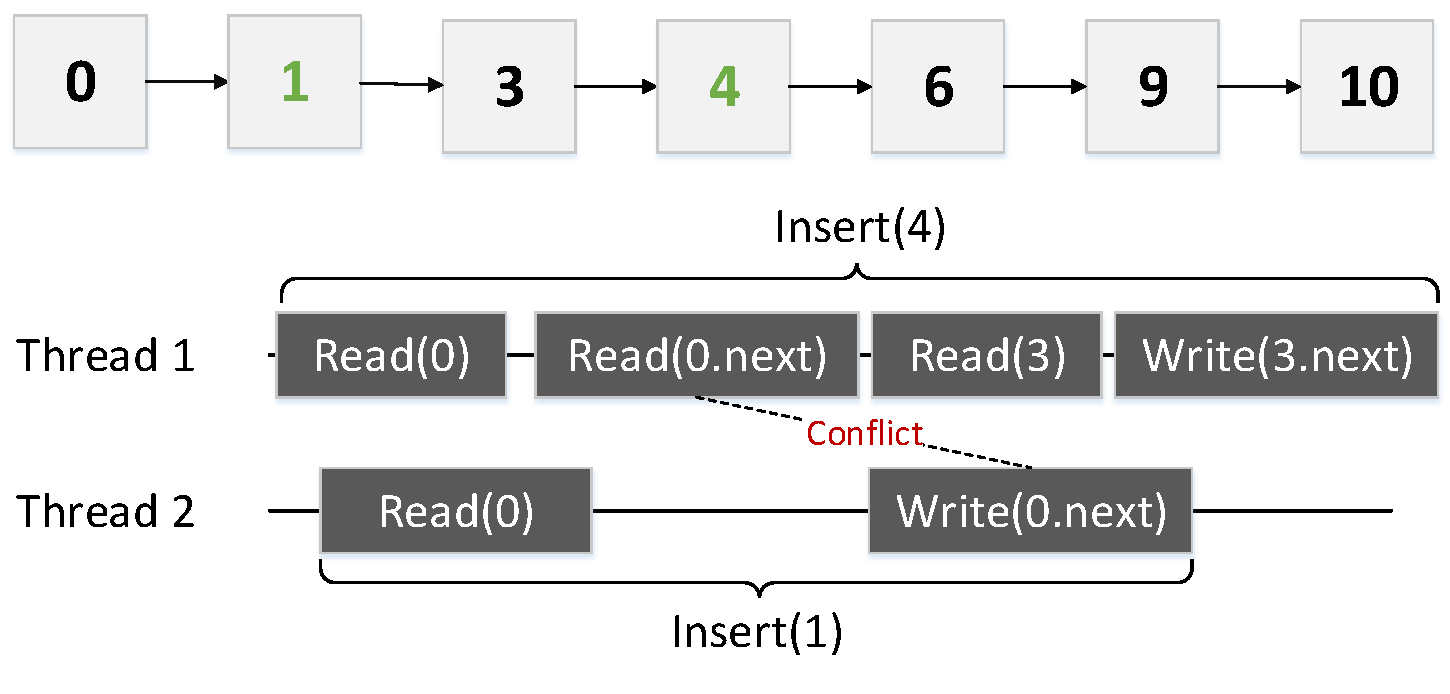
\includegraphics[width=0.6\textwidth]{stmconflict.pdf}
        \end{figure}
    }
\end{overlayarea}
\end{frame}

\begin{frame} \frametitle{Transactional Boosting \textcolor{gray}{[Herlihy and Koskinen, 2008]}}
    \begin{block}{}
        \small
        Transactional boosting uses \emph{abstract lock} to ensure that non-commutative method calls never occur concurrently. A transaction makes a sequence of invocation to the objects methods after acquiring the abstract lock associated with each one. It aborts when failed to acquire a lock and recovers from failure by invoking the \emph{inverses} of already executed operations.
    \end{block}
    \begin{itemize}
        \item<1-> Use of locks degrades the progress guarantee of lock-free data structures 
        \item<2> Upon transaction failure the rollback process causes overhead
    \end{itemize}
    \begin{overlayarea}{\textwidth}{.40\textheight}
        \centering
        \visible<2>{
            \begin{figure}[h]
                \centering
                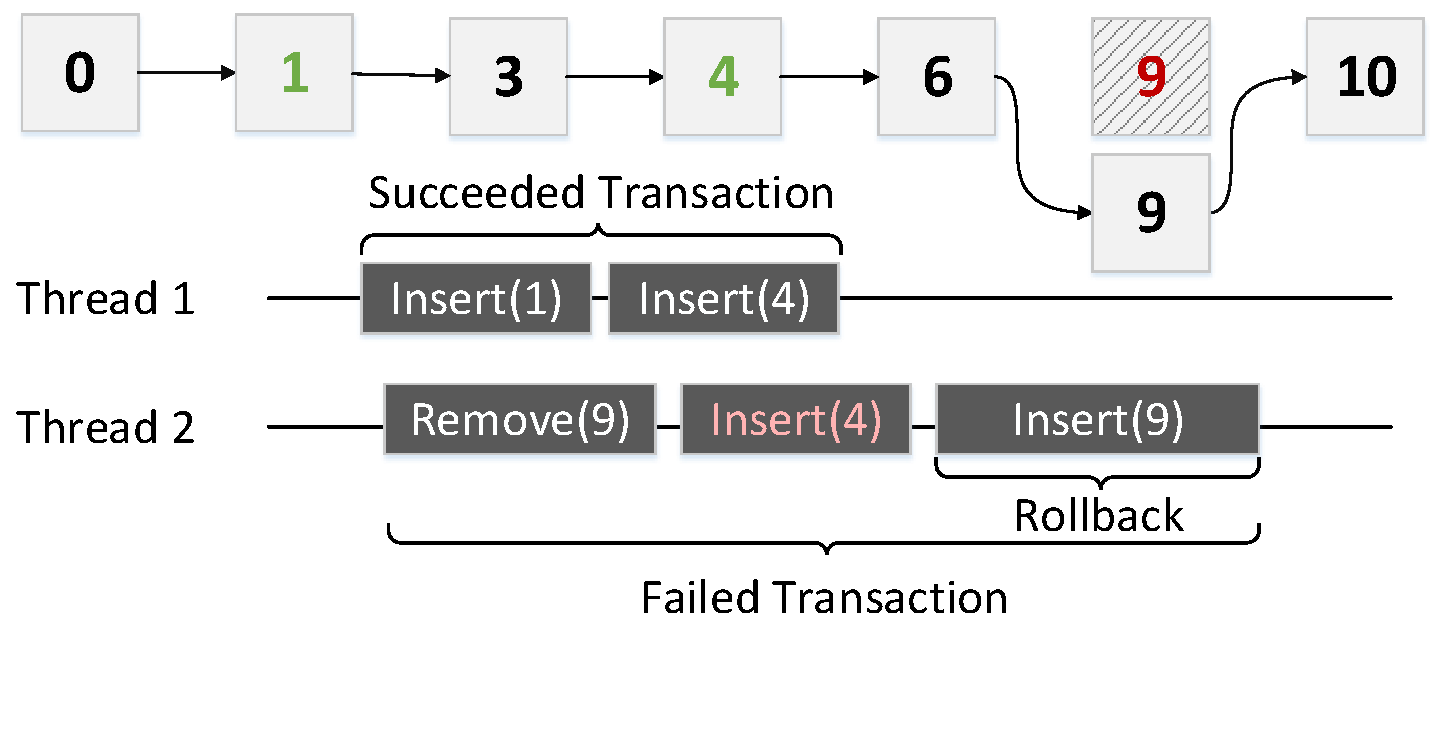
\includegraphics[width=0.6\textwidth]{boosting.pdf}
            \end{figure}
        }
    \end{overlayarea}
\end{frame}

\begin{frame} \frametitle{Automatic Semantic Locking \textcolor{gray}{[Golan-Gueta et al, 2015]}}
    \begin{block}{}
        \small
        Automatically enforces atomicity of given code fragments (multiple calls to different data structures) by inserting pessimistic \emph{abstract locks}.
    \end{block}
    \begin{figure}[h]
        \centering
        \includegraphics<1->[width=1\textwidth]{lock-inference.png}
    \end{figure}
    \begin{itemize}
        %\item<2> Use of locks degrades lock-freedom
        \item<2> Need additional container to store key-lock map
        \item<2> Lock acquiring is reordered to avoid rollbacks 
        %\item<2> Require static analysis and special compiler 
    \end{itemize}

\end{frame}

\section{Methodology}
\subsection{Overview}
\begin{frame} \frametitle{Lock-free Transactional Transformation (LFTT)}
    \begin{itemize}
        \item Challenges
            \begin{itemize}
                \item Buffering write operations
                \item Rollback failed transactions
            \end{itemize}
        \item<2-> Key contributions
            \begin{itemize}
                \item Lock-free semantic conflict detection
                \item Logical status interpretation eliminates rollbacks
                \item Cooperative transaction execution minimizes aborts
            \end{itemize}
        \item<3> Applicable data structures
            \begin{itemize}
                \item Set: Insert(k), Delete(k), Find(k)
                \item Linked data structures: list, skiplist, trees
                %\item Common fields: $key, val, next[]$
            \end{itemize}
    \end{itemize}
\end{frame}

\subsection{Algorithms}
\begin{frame} \frametitle{Node-based Conflict Detection}
    \begin{columns}
        \begin{column}{6cm}
            \begin{figure}[h]
                \centering
                \includegraphics<1->[width=1.0\textwidth]{nodeconflict}
            \end{figure}
        \end{column}
        \begin{column}{6cm}
            \begin{itemize}
                \item Embed \textsc{NodeInfo} as a monitors
                \item \textsc{TxDesc} contains operation context and status
                \item<2> Eager detection
                \item<2> Key access = node access
            \end{itemize}
        \end{column}
    \end{columns}
\end{frame}

\begin{frame} \frametitle{Transformed \textsc{Insert} Workflow}
    \begin{columns}
        \begin{column}{7cm}
            \begin{figure}[h]
                \centering
                \includegraphics<1->[width=0.9\textwidth]{lfttapplication}
            \end{figure}
        \end{column}
        \begin{column}{5cm}
            \begin{itemize}
                \item Extract \textsc{Do\_LocatePred}, and \textsc{Do\_Insert}
                \item New code path to update \textsc{NodeInfo}
                %\item Transform by applying code template
            \end{itemize}
        \end{column}
    \end{columns}
\end{frame}

\begin{frame} \frametitle{\textsc{UpdateNodeInfo} Workflow for \textsc{Insert}}
    \begin{columns}
        \begin{column}{7cm}
            \begin{figure}[h]
                \centering
                \includegraphics<1->[width=1.0\textwidth]{updatenodeinfo}
            \end{figure}
        \end{column}
        \begin{column}{5cm}
            \begin{itemize}
                \item Physically remove node with marked \textsc{NodeInfo}
                \item Enforce serialization through helping
                \item Interpret logical status using \textsc{IsKeyExisit}
                \item Returns a tri-state value
            \end{itemize}
        \end{column}
    \end{columns}
\end{frame}

\begin{frame} \frametitle{Interpretation-based Logical Rollback}
\begin{table}[h]\small
    \centering
    \caption{\textsc{IsKeyExist} Predicate}
    \begin{tabularx}{1.0\textwidth}{c|c|c|c}
        \toprule[1.5pt]
        \backslashbox{Operation}{TxStatus} & Committed & Aborted & Active \\
        \midrule
        Insert & True & False & True (same transaction)\\
        Delete & False & True & False (same transaction) \\
        Find & True & True & True \\
        \bottomrule[1.5pt]
    \end{tabularx}
\end{table}
\end{frame}

\begin{frame} \frametitle{Cooperative Transaction Execution}
    \begin{itemize}
        \item Process 
            \begin{itemize}
                \item Invoke the sequence of operation in \textsc{TxDesc}
                \item Update the transaction status using CAS
                \item Mark \textsc{NodeInfo} on successfully deleted nodes
            \end{itemize}
        \item<2> Nuances 
            \begin{itemize}
                \item Cyclic dependency check and recovery
                    \begin{itemize}
                        \item Duplicate descriptor in \textsc{HelpStack}
                    \end{itemize}
                \item No help = obstruction-freedom
                    \begin{itemize}
                        \item Contention management: aggressive, polite, karma
                    \end{itemize}

            \end{itemize}
    \end{itemize}
\end{frame}

\begin{frame} \frametitle{LFTT in Action}
    \begin{figure}[h]
        \centering
        \includegraphics<1>[width=1\textwidth]{lfttconflict}
        \includegraphics<2>[width=1\textwidth]{lfttconflict1}
    \end{figure}
\end{frame}

\section{Experiment}
\subsection{Setup}
\begin{frame} \frametitle{Environment}
    \begin{itemize}
        \item Hardware
            \begin{itemize}
                \item 64-core NUMA (4 AMD Opteron @2.1GHz)
                %\item 6-core (12 w/ Hyper-threading) SMP (Intel Xeon @2.9GHz)
            \end{itemize}
        \item Micro-benchmark
            \begin{itemize}
                \item GCC 4.7 w/ O3
                \item 1, 2, 4, 8, and 16 operations per transaction
                \item Write-dominated, read-dominated, and mixed workloads
            \end{itemize}
    \end{itemize}
\end{frame}

\begin{frame} \frametitle{Alternatives}
    \begin{itemize}
        \item Transactional skiplist \textcolor{gray}{[Fraser, 2004]}
            \begin{itemize}
                \item Object-based STM (OTM) \textcolor{gray}{[Fraser, 2004]}
                \item Transactional boosting (BST) 
                \item Lock-free Transactional Transformation (LFT)
            \end{itemize}
        \item Transactional linked list \textcolor{gray}{[Harris, 2001]}
            \begin{itemize}
                \item Norec word-based STM (NTM) \textcolor{gray}{[Dalessandro, 2010]}
                \item Transactional boosting (BST)
                \item Lock-free Transactional Transformation (LFT)
            \end{itemize}
    \end{itemize}
\end{frame}

\subsection{Performance}
\begin{frame} \frametitle{Throughput --- Skiplist Mixed Workload}
    \begin{columns}
        \begin{column}{8cm}
            \begin{figure}[t]
                \centering
                \includegraphics<1>[width=1\columnwidth]{amdskip33ins10kfilled2.pdf}
                \includegraphics<2>[width=1\columnwidth]{amdskip33ins10kfilled4.pdf}
                \includegraphics<3>[width=1\columnwidth]{amdskip33ins10kfilled8.pdf}
                \includegraphics<4>[width=1\columnwidth]{amdskip33ins10kfilled16.pdf}
                \includegraphics<5>[width=1\columnwidth]{amdskip33ins10kfilled.pdf}
                \caption{1M Key, 33\% \textsc{Insert}, 33\% \textsc{Delete}, 34\% \textsc{Find}}
                \end{figure}
            \end{column}
            \begin{column}{4.3cm}
                \begin{itemize}
                    \item Average of 60\% speedup over boosting 
                    \item 3 times speedup over STM
                    \item No spurious aborts
                \end{itemize}
            \end{column}
        \end{columns}
\end{frame}

%\begin{frame} \frametitle{Throughput --- Skiplist Read-dominated Workload}
    %\begin{columns}
        %\begin{column}{8cm}
            %\begin{figure}[t]
                %\centering
                %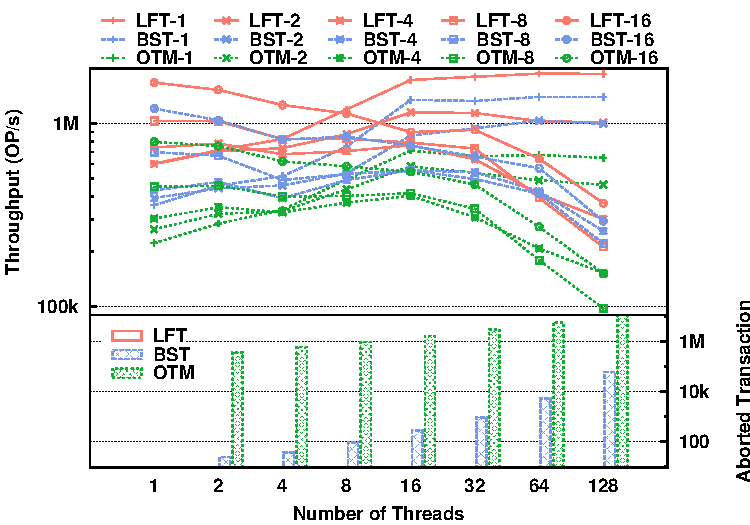
\includegraphics[width=1\columnwidth]{amdskip15ins10kfilled.pdf}
                %\caption{1M Key, 15\% \textsc{Insert}, 5\% \textsc{Delete}, 80\% \textsc{Find}}
                %\end{figure}
            %\end{column}
            %\begin{column}{4.3cm}
                %\begin{itemize}
                    %\item Up to 125\% speedup over boosting 
                    %\item 3 times speedup over STM
                    %\item No spurious aborts
                %\end{itemize}
            %\end{column}
        %\end{columns}
%\end{frame}

\begin{frame} \frametitle{Throughput --- Linked List Mixed Workload}
    \begin{columns}
        \begin{column}{8cm}
            \begin{figure}[t]
                \centering
                \includegraphics<1>[width=1\columnwidth]{amd33ins10kfilled2.pdf}
                \includegraphics<2>[width=1\columnwidth]{amd33ins10kfilled4.pdf}
                \includegraphics<3>[width=1\columnwidth]{amd33ins10kfilled8.pdf}
                \includegraphics<4>[width=1\columnwidth]{amd33ins10kfilled16.pdf}
                \includegraphics<5>[width=1\columnwidth]{amd33ins10kfilled.pdf}
                \caption{10K Key, 33\% \textsc{Insert}, 33\% \textsc{Delete}, 34\% \textsc{Find}}
                \end{figure}
            \end{column}
            \begin{column}{4.3cm}
                \begin{itemize}
                    \item Average of 40\% speedup over boosting
                    \item 10 times speedup over STM
                    \item 2 to 3 orders of magnitude less spurious aborts
                \end{itemize}
            \end{column}
        \end{columns}
\end{frame}

\section{Conclusion}
\begin{frame} \frametitle{Summary}
    \begin{itemize}
        \item LFTT characteristics
            \begin{itemize}
                \item Built-in transaction support for lock-free sets
                \item Excels at large transactions
                \item Greater success rate with minimal spurious aborts
            \end{itemize}
        %\item Support wait-free data structures
            %\begin{itemize}
                %\item Wait-free update of \textsc{TxInfo}
                %\item Wait-free memory management 
            %\end{itemize}
        \item Future work
            \begin{itemize}
                \item Support map abstract data type
                \item Support wait-free data structures
            \end{itemize}
        \item Library of transactional data structures
            \begin{itemize}
                \item Cross-container transactions
                \item http://cse.eecs.ucf.edu/gitlab/deli/libtxd
            \end{itemize}
    \end{itemize}
\end{frame}

%\begin{frame}[shrink=35] \frametitle{Thank You!}
%%\bibliographystyle{abbrv}
%%\bibliography{citation}
%\printbibliography[heading=subbibliography,title={References}]
%\end{frame}

\end{document}
